%* 
%* ------------------------------------------------------------------
%* PanelInstruments.tex - Using the Panel Instruments Widgets
%* Created by Robert Heller on Thu Apr 19 14:43:50 2007
%* ------------------------------------------------------------------
%* Modification History: $Log$
%* Modification History: Revision 1.2  2007/11/30 13:56:50  heller
%* Modification History: Novemeber 30, 2007 lockdown.
%* Modification History:
%* Modification History: Revision 1.1  2007/05/06 12:49:39  heller
%* Modification History: Lock down  for 2.1.8 release candidate 1
%* Modification History:
%* Modification History: Revision 1.1  2002/07/28 14:03:50  heller
%* Modification History: Add it copyright notice headers
%* Modification History:
%* ------------------------------------------------------------------
%* Contents:
%* ------------------------------------------------------------------
%*  
%*     Model RR System, Version 2
%*     Copyright (C) 1994,1995,2002-2005  Robert Heller D/B/A Deepwoods Software
%* 			51 Locke Hill Road
%* 			Wendell, MA 01379-9728
%* 
%*     This program is free software; you can redistribute it and/or modify
%*     it under the terms of the GNU General Public License as published by
%*     the Free Software Foundation; either version 2 of the License, or
%*     (at your option) any later version.
%* 
%*     This program is distributed in the hope that it will be useful,
%*     but WITHOUT ANY WARRANTY; without even the implied warranty of
%*     MERCHANTABILITY or FITNESS FOR A PARTICULAR PURPOSE.  See the
%*     GNU General Public License for more details.
%* 
%*     You should have received a copy of the GNU General Public License
%*     along with this program; if not, write to the Free Software
%*     Foundation, Inc., 675 Mass Ave, Cambridge, MA 02139, USA.
%* 
%*  
%* 

\chapter{Using the Panel Instruments Widgets}
\label{chapt:PanelInstruments}
\typeout{$Id$}
\lstinputlisting[caption={Using the Panel Instrument based widgets},
		 label={lst:PI:SampleCodeInstrumentPanel},
		 firstline=38]{SampleCodeInstrumentPanel.tcl}
\begin{figure}[hbpt]
\begin{centering}
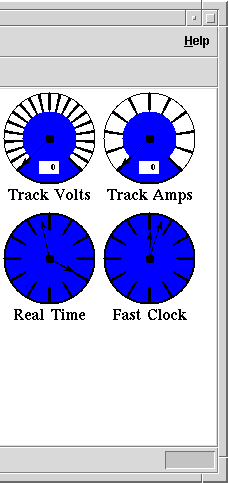
\includegraphics{PanelInstrument.png}
\caption{Some Panel Instruments}
\label{fig:PI:PanelInstrument}
\end{centering}
\end{figure}
Listing~\ref{lst:PI:SampleCodeInstrumentPanel} contains code to create
some of the panel instrument widgets.  The window this code helped to
create is shown in Figure~\ref{fig:PI:PanelInstrument}. Several typical
panel instruments are shown with the code to create them.

